\chapter{Thiết Kế, Lắp Đặt Và Đánh Giá Hệ Thống}

\section{Thiết kế kiến trúc hệ thống}
\subsection{Kiến trúc tổng thể}
Hệ thống quan trắc chất lượng không khí được thiết kế dưới dạng một nút đo IoT hoàn chỉnh. Cấu trúc phần cứng được chia làm 6 khối chức năng chính xoay quanh bộ vi xử lý trung tâm ESP32:
\begin{enumerate}
    \item \textbf{Khối xử lý trung tâm (ESP32 DevKit)}: Thực hiện việc lấy mẫu dữ liệu từ cảm biến, quản lý trạng thái hệ thống, hiển thị màn hình, lưu trữ offline flash và truyền HTTPS lên Supabase.
    \item \textbf{Khối cảm biến}: Gồm DHT22 (Nhiệt độ/Độ ẩm), MQ135 (Khí gas/CO2), GP2Y1010AU0F (Bụi mịn).
    \item \textbf{Khối buồng đo lấy mẫu khí chủ động}: Gồm quạt hút 5V lắp đặt trong buồng đo cơ khí. Quạt hút được điều khiển tắt/bật thông qua Relay để chủ động định lượng lượng khí lưu thông qua cảm biến.
    \item \textbf{Khối nguồn}: Sử dụng cổng DC 5V kết hợp mạch UPS dự phòng cấp nguồn 5V/3.3V ổn định cho hệ thống.
    \item \textbf{Khối hiển thị tại chỗ}: Màn hình OLED SSD1306 0.96 inch hiển thị thông số và trạng thái mạng.
    \item \textbf{Khối cảnh báo cục bộ}: Đèn LED đỏ và còi buzzer cảnh báo tại chỗ khi chỉ số ô nhiễm vượt ngưỡng.
\end{enumerate}

\subsection{Sơ đồ luồng tín hiệu và luồng điều khiển}
\begin{itemize}
    \item \textbf{Luồng dữ liệu (Data Flow)}: Cảm biến $\rightarrow$ Đọc ADC/Digital $\rightarrow$ Lọc nhiễu trung bình $\rightarrow$ Đóng gói JSON $\rightarrow$ Đẩy lên Supabase (hoặc ghi cache SPIFFS khi mất mạng).
     \begin{figure}[H]
        \centering
        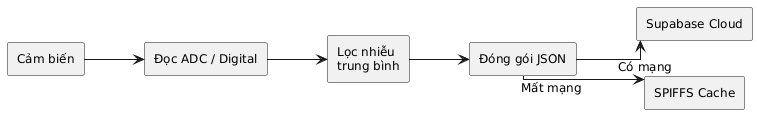
\includegraphics[
            width=0.8\textwidth,
            height=0.28\textheight,
            keepaspectratio
        ]{images/dataflow.png}
        \caption{Sơ đồ luồng dữ liệu}
        \label{fig:dataflow}
    \end{figure}
    \item \textbf{Luồng điều khiển (Control Flow)}: 
  \begin{itemize}
      \item Đọc nút bấm $\rightarrow$ Kích hoạt ngắt ngoài $\rightarrow$ Đánh thức \texttt{TaskSensors} thức dậy đo đạc ngay lập tức.
      \item Dữ liệu vượt ngưỡng $\rightarrow$ Kéo chân \texttt{WARNING\_LED\_PIN} và \texttt{BUZZER\_PIN} lên mức HIGH theo chu kỳ trễ để phát tín hiệu.
      \item Edge Function (Supabase) $\rightarrow$ Trình quét Webhook $\rightarrow$ PostgREST $\rightarrow$ Gửi tin nhắn Telegram Bot API.
      \begin{figure}[H]
        \centering
        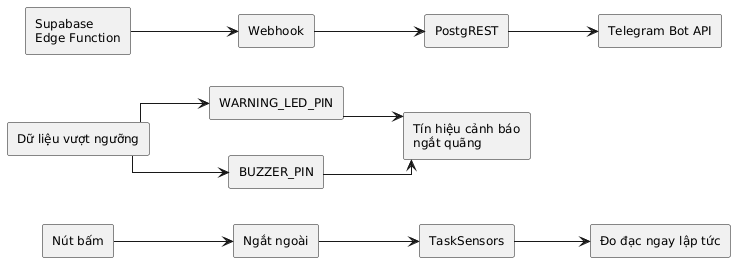
\includegraphics[
            width=0.8\textwidth,
            height=0.5\textheight,
            keepaspectratio
        ]{images/controlflow.png}
        \caption{Luồng điều khiển}
        \label{fig:controlflow}
    \end{figure}
    \end{itemize}
     
\end{itemize}

\section{Thiết kế phần cứng}
\subsection{Sơ đồ chân GPIO kết nối thực tế}
Các chân kết nối vật lý trên bo mạch ESP32 được cấu hình chính xác theo file mã nguồn \texttt{Config.h} để tránh xung đột phần cứng. Chi tiết phân phối chân GPIO được mô tả trong Bảng \ref{tab:gpioallocation}.

\begin{table}[H]
\centering
\caption{Bảng phân bổ chân GPIO trên vi điều khiển ESP32}
\label{tab:gpioallocation}
\footnotesize
\renewcommand{\arraystretch}{1.35}
\setlength{\tabcolsep}{4pt}

\begin{tabularx}{\textwidth}{|p{3.0cm}|c|p{2.5cm}|p{3.0cm}|X|}
\hline
\textbf{Tên Pin cấu hình} 
& \textbf{Chân GPIO} 
& \textbf{Kiểu kết nối} 
& \textbf{Thiết bị ngoại vi} 
& \textbf{Giao tiếp / Vai trò} \\
\hline

\texttt{DHTPIN} 
& 14 
& Digital Input 
& Cảm biến DHT22 
& Giao thức 1-wire, dùng để đọc nhiệt độ và độ ẩm môi trường. \\
\hline

\texttt{MQ135\_PIN} 
& 34 
& Analog Input 
& Cảm biến MQ135 
& ADC1\_CH6, dùng để đọc điện áp tương ứng với mức khí gas tổng quát. \\
\hline

\texttt{GP2Y\_PIN} 
& 35 
& Analog Input 
& Cảm biến bụi GP2Y 
& ADC1\_CH7, dùng để đọc tín hiệu analog biểu diễn mức bụi tương đối. \\
\hline

\texttt{GP2Y\_LED\_PIN} 
& 25 
& Digital Output 
& Cảm biến bụi GP2Y 
& Điều khiển LED hồng ngoại bên trong cảm biến, hoạt động mức thấp (Active LOW). \\
\hline

\texttt{WARNING\_LED\_PIN} 
& 26 
& Digital Output 
& LED màu đỏ 
& Phát tín hiệu cảnh báo tại chỗ khi dữ liệu vượt ngưỡng thiết lập. \\
\hline

\texttt{BUZZER\_PIN} 
& 27 
& Digital Output 
& Còi buzzer 5V 
& Phát cảnh báo âm thanh tại chỗ khi hệ thống ở trạng thái cảnh báo. \\
\hline

\texttt{RELAY\_PIN} 
& 16 
& Digital Output 
& Relay điều khiển 5V 
& Điều khiển đóng/cắt nguồn cho quạt lấy mẫu khí và khối buồng đo. \\
\hline

\texttt{BUTTON\_PIN} 
& 4 
& Digital Input 
& Nút bấm cơ học 
& Ngõ vào phục vụ thao tác thủ công hoặc đánh thức hệ thống bằng ngắt ngoài. \\
\hline

\texttt{I2C\_SDA} 
& 21 
& I2C Bus line 
& OLED SSD1306 
& Đường truyền dữ liệu SDA của giao tiếp I2C. \\
\hline

\texttt{I2C\_SCL} 
& 22 
& I2C Bus line 
& OLED SSD1306 
& Đường truyền xung nhịp SCL của giao tiếp I2C. \\
\hline

\end{tabularx}
\end{table}

\begin{figure}[H]
        \centering
        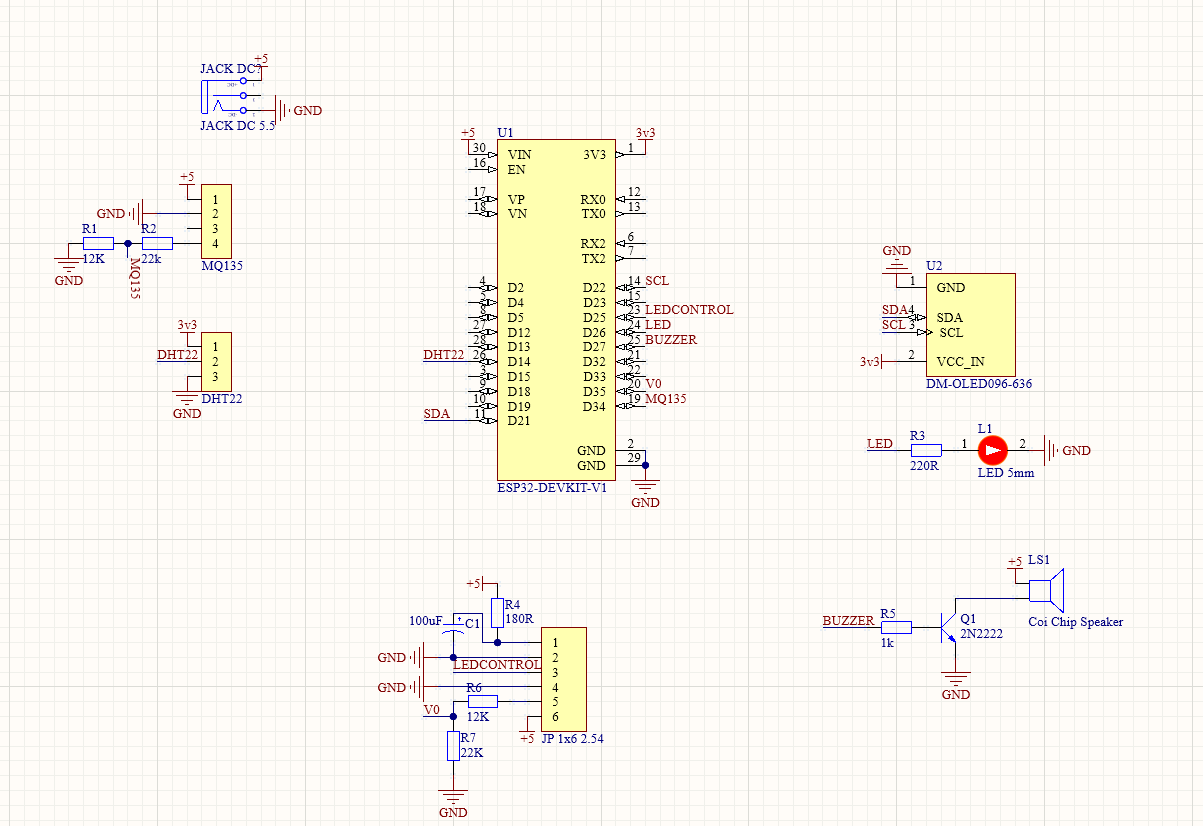
\includegraphics[
            width=0.8\textwidth,
            height=0.5\textheight,
            keepaspectratio
        ]{images/machaltium.png}
        \caption{Hình ảnh mạch mô phỏng trên altium}
        \label{fig:circuitaltium}
    \end{figure}

\begin{figure}[H]
        \centering
        \includegraphics[
            width=0.8\textwidth,
            height=0.5\textheight,
            keepaspectratio
        ]{images/pcb_circuit.png}
        \caption{Thiết kế PCB layout}
        \label{fig:pcblayout}
    \end{figure}

\subsection{Thiết kế mạch nguồn, buồng đo khí cải tiến và cầu phân áp}
\textbf{Thiết kế mạch nguồn}: Các cảm biến MQ135 và GP2Y yêu cầu nguồn 5V dòng cao, trong khi ESP32 hoạt động ở mức logic 3.3V. Trên PCB, nhóm thiết kế mạch nguồn cách ly sử dụng diode chống dòng ngược và các tụ lọc nguồn lớn (100uF và 10nF) để triệt tiêu nhiễu sụt áp khi Wi-Fi ESP32 phát sóng hoặc quạt hút khởi động.

\textbf{Buồng lấy mẫu khí chủ động}: Để tránh hiện tượng đo sai lệch do cảm biến tỏa nhiệt làm thay đổi nhiệt độ xung quanh hoặc luồng khí thổi tự do không đều, nhóm thiết kế một buồng đo cơ khí kín bằng nhựa acrylic. Lối vào buồng đo có thiết kế phễu định hình, lối ra lắp đặt quạt hút 5V dòng thấp. Quạt hút hoạt động đồng bộ với Relay điều khiển qua chân \texttt{RELAY\_PIN} thông qua transistor S8050 bảo vệ đệm. Quạt chỉ chạy trong chu kỳ WARMUP (60s) để chủ động hút không khí mới từ môi trường ngoài chạy qua bề mặt cảm biến với lưu lượng ổn định, sau đó tự động tắt trong trạng thái IDLE để tiết kiệm năng lượng.
  Do chân ADC của ESP32 chỉ chịu được điện áp tối đa 3.3V, trong khi đầu ra Analog của MQ135 chạy ở mức 5V, nhóm thiết kế cầu phân áp trên PCB gồm hai điện trở $R1 = 12k\Omega$ và $R2 = 22k\Omega$ kết nối từ đầu ra cảm biến xuống GND. Điện áp đọc được tại chân ADC ESP32 ($V_{ADC}$) sẽ được quy đổi ngược lại điện áp thực tế đầu ra cảm biến ($V_{sensor}$) thông qua công thức cầu phân áp:
  \begin{equation}
      V\_{sensor} = V\_{ADC} \times \frac{R1 + R2}{R2} = V\_{ADC} \times \frac{12 + 22}{22} = V\_{ADC} \times 1.545
  \end{equation}
  Giá trị hệ số cầu phân áp này khớp chính xác với định nghĩa \texttt{\#define VOLTAGE\_DIVIDER\_FACTOR 1.545} trong cấu hình \texttt{Config.h}.

\section{Thiết kế firmware}
\subsection{Cấu trúc project PlatformIO}
Mã nguồn dự án được tổ chức cấu trúc module hóa rõ ràng trên PlatformIO:
\begin{itemize}
    \item \texttt{include/Config.h}: Chứa sơ đồ chân GPIO, hằng số cấu hình và cấu trúc bản ghi \texttt{SensorRecord}.
    \item \texttt{include/secrets.h}: Chứa thông tin đăng nhập Wi-Fi và API Key của Supabase (được ignore khỏi git).
    \item \texttt{src/drivers/Display.cpp} / \texttt{Display.h}: Driver điều khiển màn hình OLED SSD1306.
    \item \texttt{src/drivers/Sensors.cpp} / \texttt{Sensors.h}: Driver cấu hình và đọc dữ liệu từ cảm biến DHT22, MQ135, GP2Y1010.
    \item \texttt{src/drivers/Indicators.cpp} / \texttt{Indicators.h}: Điều khiển LED và còi buzzer cảnh báo.
    \item \texttt{src/app/Cloud.cpp} / \texttt{Cloud.h}: Xử lý kết nối Wi-Fi, OTA và gửi dữ liệu Supabase qua HTTPS POST.
    \item \texttt{src/app/DataManager.cpp} / \texttt{DataManager.h}: Quản lý đọc, ghi và xử lý offline cache trên SPIFFS.
    \item \texttt{src/main.cpp}: Khởi tạo hệ thống và phối hợp các task FreeRTOS.
\end{itemize}

\subsection{Chi tiết hoạt động các Task FreeRTOS}
Firmware điều khiển chạy đồng thời 3 task FreeRTOS được điều phối bởi hệ điều hành nhúng:
\begin{itemize}
    \item \textbf{TaskSensors (Core 1, Priority 2)}: 
\end{itemize}
  Governs máy trạng thái của hệ thống. Chu kỳ lặp mặc định là 5 phút:
  1. Kéo chân \texttt{RELAY\_PIN} lên HIGH để bật nguồn buồng đo và quạt hút.
  2. Đếm ngược 60 giây warm-up trên OLED.
  3. Gọi hàm \texttt{sensors.readAll()} để đọc các cảm biến.
  4. Lấy khóa \texttt{dataMutex} để cập nhật dữ liệu vào biến toàn cục \texttt{sharedRecord}, sau đó nhả mutex.
  5. Gửi tín hiệu thông báo (Task Notification) cho \texttt{TaskNetwork} biết dữ liệu mới đã sẵn sàng.
  6. Kéo chân \texttt{RELAY\_PIN} xuống LOW để tắt quạt hút và chuyển sang ngủ tiết kiệm điện (vTaskDelay) trong 5 phút.
\begin{itemize}
    \item \textbf{TaskOLED (Core 1, Priority 1)}:
\end{itemize}
  Thực hiện vẽ lại màn hình OLED mỗi 1 giây. Task lấy khóa \texttt{dataMutex} để đọc an toàn các chỉ số đo hiện tại từ \texttt{sharedRecord}, hiển thị lên OLED theo giao diện xoay vòng (Trang 1: Nhiệt độ/Độ ẩm, Trang 2: Bụi mịn/Khí MQ135, Trang 3: Trạng thái kết nối và IP Address). Việc lấy vẽ màn hình phải lấy khóa \texttt{i2cMutex} để đảm bảo bus I2C không bị tranh chấp với task sensors.
\begin{itemize}
    \item \textbf{TaskNetwork (Core 0, Priority 1)}:
\end{itemize}
  Chờ tín hiệu thông báo từ \texttt{TaskSensors}. Khi có dữ liệu mới:
  1. Kiểm tra trạng thái kết nối Wi-Fi. Nếu mất kết nối, thực hiện reconnect tự động trong tối đa 10 giây (cơ chế reconnect thông minh không chặn hệ thống).
  2. Nếu kết nối Wi-Fi thành công, task tiến hành kiểm tra xem có tệp tin \texttt{/cache.txt} trong SPIFFS chứa dữ liệu tích lũy offline hay không. Nếu có, task sẽ đọc từng dòng JSON, chuyển đổi ngược và gọi \texttt{cloud.publishToSupabase(record)} để đẩy bù dữ liệu lên Supabase.
  3. Gửi bản ghi hiện tại lên Supabase. Nếu gửi thành công, kết thúc chu kỳ.
  4. Nếu Wi-Fi mất hoặc HTTP POST thất bại (ví dụ: lỗi mạng hoặc database bảo trì), task tự động gọi \texttt{dataManager.cacheRecord(record)} để lưu bản ghi vào bộ nhớ flash ngoại tuyến thông qua hệ thống SPIFFS.

\section{Xây dựng nguyên mẫu thử nghiệm (Prototype)}
Thiết bị nguyên mẫu thử nghiệm được hoàn thiện lắp ráp tích hợp đầy đủ trong buồng đo cơ khí. Bo mạch PCB được đặt gia công và hàn đầy đủ linh kiện.
\insertimage{images/anhsanpham.png}{Hệ thống đo chất lượng không khí hoàn thiện}{fig:prototypehust}

Vỏ hộp buồng đo khí được chế tạo bằng nhựa cứng cách điện, có quạt lấy mẫu định lượng hút khí từ phễu nạp dẫn qua cảm biến bụi Sharp và MQ135 trước khi xả ra ngoài. OLED SSD1306 được bố trí ở mặt trước để người dùng tiện theo dõi trực quan tại chỗ.

\section{Kiểm thử hệ thống (Verification \& Testing)}
Nhóm đã tiến hành kiểm thử toàn diện hệ thống nhúng thông qua các kịch bản test case chức năng và phi chức năng được mô tả trong Bảng \ref{tab:testcases}.

\begin{table}[H]
\centering
\caption{Bảng kết quả kiểm thử chức năng và phi chức năng của hệ thống}
\label{tab:testcases}
\small
\renewcommand{\arraystretch}{1.35}
\setlength{\tabcolsep}{5pt}

\begin{tabularx}{\textwidth}{|p{1.8cm}|p{3.6cm}|X|p{1.5cm}|}
\hline
\textbf{Mã Test} 
& \textbf{Kịch bản kiểm thử} 
& \textbf{Kết quả mong đợi} 
& \textbf{Đánh giá} \\
\hline

\textbf{TC-01} 
& Khởi động và Warm-up 
& Relay bật, quạt quay, OLED hiển thị đếm ngược 60 giây làm nóng cảm biến. 
& Đạt \\
\hline

\textbf{TC-02} 
& Đọc dữ liệu 
& Đọc chính xác nhiệt độ, độ ẩm, MQ135 và bụi GP2Y. Cập nhật OLED thành công. 
& Đạt \\
\hline

\textbf{TC-03} 
& Ngắt nút bấm vật lý 
& Nhấn nút GPIO 4 lập tức đánh thức hệ thống dậy đo đạc mà không cần chờ hết 5 phút. 
& Đạt \\
\hline

\textbf{TC-04} 
& Cảnh báo cục bộ vượt ngưỡng 
& Đốt thử gas nhẹ gần buồng đo $\rightarrow$ buzzer phát âm thanh cảnh báo, LED nháy đỏ liên tục. 
& Đạt \\
\hline

\textbf{TC-05} 
& Gửi dữ liệu Supabase 
& Post dữ liệu qua mạng Wi-Fi $\rightarrow$ bảng database Supabase xuất hiện dòng log mới sau $< 2~\mathrm{s}$. 
& Đạt \\
\hline

\textbf{TC-06} 
& Kiểm thử ngắt mạng (Offline) 
& Tắt bộ phát Wi-Fi khi thiết bị đang đo $\rightarrow$ thiết bị tự động ghi nhận bản ghi vào SPIFFS \texttt{/cache.txt}. 
& Đạt \\
\hline

\textbf{TC-07} 
& Kiểm thử khôi phục kết nối 
& Bật lại Wi-Fi $\rightarrow$ thiết bị tự động đọc \texttt{/cache.txt}, đẩy bù các bản ghi cũ lên database thành công. 
& Đạt \\
\hline

\textbf{TC-08} 
& Watchdog Timer 
& Gây nghẽn nhân tạo làm đơ chương trình $\rightarrow$ Watchdog phát hiện sau 15 giây và restart ESP32 an toàn. 
& Đạt \\
\hline

\end{tabularx}
\end{table}

\subsection{Bằng chứng kết quả chạy thực nghiệm tại chỗ và Cloud}
Để chứng minh hệ thống hoạt động đúng kịch bản thiết kế, nhóm lưu lại các hình ảnh thực tế từ màn hình hiển thị OLED, các dòng thông tin truyền nhận Serial Monitor, cơ sở dữ liệu Supabase và tin nhắn cảnh báo gửi về Telegram:

\begin{figure}[H]
    \centering
    \begin{minipage}{0.48\textwidth}
        \centering
        \IfFileExists{images/oledscreenshot.png}{
            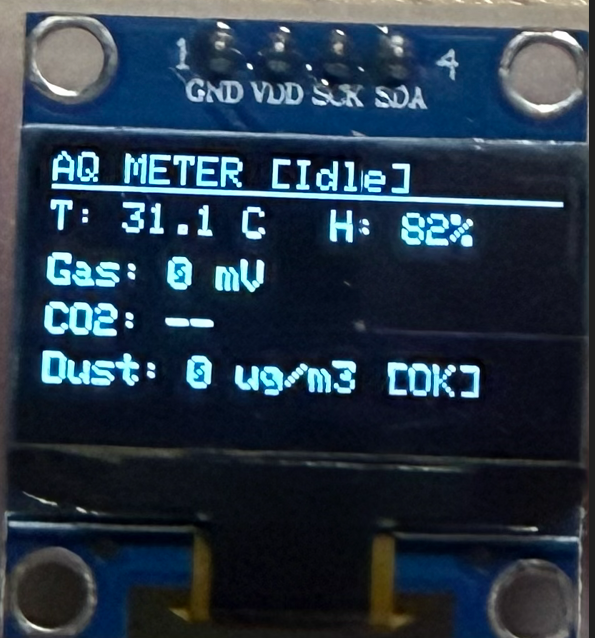
\includegraphics[width=\textwidth]{images/oledscreenshot.png}
        }{
            \setlength{\fboxsep}{10pt}
            \setlength{\fboxrule}{1.0pt}
            \fbox{
                \begin{minipage}{0.9\textwidth}
                    \centering
                    \vspace{1.0cm}
                    \textcolor{red}{\textbf{[ẢNH CHỤP OLED]}} \\
                    \vspace{0.3cm}
                    \textit{Bổ sung file tại:} \\
                    \texttt{images/oledscreenshot.png}
                    \vspace{1.0cm}
                \end{minipage}
            }
        }
        \caption{Ảnh chụp màn hình hiển thị OLED thực tế}
        \label{fig:oledscreenshot}
    \end{minipage}
    \hfill
    \begin{minipage}{0.48\textwidth}
        \centering
        \IfFileExists{images/serialmonitor.png}{
            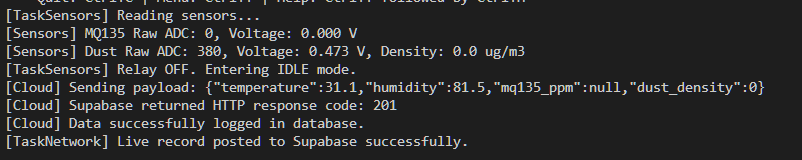
\includegraphics[width=\textwidth]{images/serialmonitor.png}
        }{
            \setlength{\fboxsep}{10pt}
            \setlength{\fboxrule}{1.0pt}
            \fbox{
                \begin{minipage}{0.9\textwidth}
                    \centering
                    \vspace{1.0cm}
                    \textcolor{red}{\textbf{[ẢNH CHỤP SERIAL]}} \\
                    \vspace{0.3cm}
                    \textit{Bổ sung file tại:} \\
                    \texttt{images/serialmonitor.png}
                    \vspace{1.0cm}
                \end{minipage}
            }
        }
        \caption{Ảnh chụp giao diện Serial Monitor (Log debug)}
        \label{fig:serialmonitor}
    \end{minipage}
    \caption{Kết quả vận hành thực tế tại chỗ của thiết bị nhúng}
    \label{fig:localoperation}
\end{figure}
Hình \ref{fig:localoperation} thể hiện kết quả chạy thực tế tại chỗ của thiết bị: Hình \ref{fig:oledscreenshot} là màn hình hiển thị OLED xoay vòng thông báo các thông số hiện thời của trạm đo; Hình \ref{fig:serialmonitor} là các dòng log gỡ lỗi (debug) kết xuất qua cổng Serial Monitor chứng minh vòng lặp các Task vận hành trơn tru.

\insertimage{images/supabasescreenshot.png}{Ảnh chụp màn hình cơ sở dữ liệu bảng air\_quality\_logs trên giao diện Supabase Console}{fig:supabasescreenshot}
Hình \ref{fig:supabasescreenshot} thể hiện bảng dữ liệu \texttt{air\_quality\_logs} lưu trữ lịch sử đo đạc thời gian thực trên Cloud Console của Supabase, ghi nhận đầy đủ các cột thông số (temperature, humidity, mq135\_ppm, dust\_density, status, warning) chèn vào cơ sở dữ liệu đúng chu kỳ.

\insertimage{images/telegramalert.png}{Ảnh chụp màn hình điện thoại nhận tin nhắn cảnh báo vượt ngưỡng gửi từ Telegram Bot}{fig:telegramalert}
Hình \ref{fig:telegramalert} minh họa tin nhắn cảnh báo khẩn cấp được gửi tự động về điện thoại của các thành viên trong nhóm thông qua Telegram Bot khi hệ thống phát hiện nồng độ khí gas độc hại hoặc bụi mịn vượt qua ngưỡng cảnh báo an toàn thiết lập.

\section{Triển khai thực nghiệm và phân tích dữ liệu chuyên sâu}
\subsection{Kết quả đo thực nghiệm}
Để đánh giá độ ổn định của hệ thống trong môi trường thực tế, nhóm đã tiến hành triển khai song song hai trạm quan trắc đo liên tục từ tháng 05/2026 đến tháng 07/2026:
\begin{itemize}
    \item \textbf{Đo trong phòng (Indoor)}: Đặt tại phòng học thí nghiệm.
    \item \textbf{Đo tại khu vực gửi xe (Outdoor)}: Đặt tại khu vực nhà xe lộ thiên, chịu ảnh hưởng trực tiếp của đợt nắng tháng 6 tại Hà Nội.
\end{itemize}

Dữ liệu lịch sử chi tiết được ghi nhận tự động vào 2 tệp tin dữ liệu: [indoor\_logs.csv] và [outdoor\_logs.csv]. Dữ liệu này chứng minh hệ thống có thể hoạt động ổn định và hiếm khi bị treo đơ hay mất mát số liệu trong suốt khoag đo thực tế nhờ cơ chế SPIFFS cache dự phòng.

\subsubsection{Kết quả đo trong phòng}
Dữ liệu đo đạc thực tế trong phòng thí nghiệm được trực quan hóa qua 4 biểu đồ đo độc lập cho từng thông số dưới đây:

\insertimage{images/indoortemp.png}{Biến thiên nhiệt độ đo được trong phòng thí nghiệm}{fig:indoortemp}

\insertimage{images/indoorhumidity.png}{Biến thiên độ ẩm tương đối đo được trong phòng thí nghiệm}{fig:indoorhumidity}

\insertimage{images/indoormq135.png}{Biến thiên nồng độ khí gas tương đối đo được trong phòng thí nghiệm}{fig:indoormq135}

\insertimage{images/indoordust.png}{Biến thiên nồng độ bụi tương đối đo được trong phòng thí nghiệm}{fig:indoordust}

\subsubsection{Kết quả đo ngoài trời khu vực nhà xe}
Dữ liệu đo đạc thực tế ngoài trời tại khu vực nhà xe ghi nhận các biến động môi trường rõ rệt và các đỉnh nắng nóng trong tháng 6:

\insertimage{images/outdoortemp.png}{Biến thiên nhiệt độ đo được tại nhà xe (đỉnh điểm đợt nắng nóng tháng 6)}{fig:outdoortemp}

\insertimage{images/outdoorhumidity.png}{Biến thiên độ ẩm tương đối đo được tại nhà xe}{fig:outdoorhumidity}

\insertimage{images/outdoormq135.png}{Biến thiên nồng độ khí gas tương đối đo được tại nhà xe (tăng vọt vào giờ cao điểm)}{fig:outdoormq135}

\insertimage{images/outdoordust.png}{Biến thiên nồng độ bụi tương đối đo được tại nhà xe}{fig:outdoordust}

\subsection{Phân tích tương quan và hiệu chuẩn cảm biến bụi bằng Machine Learning}
Cảm biến bụi quang học giá rẻ GP2Y1010AU0F dễ bị sai số lớn dưới tác động của độ ẩm không khí do hiện tượng hút ẩm hạt nước trong buồng đo. Để giải quyết triệt để vấn đề này, nhóm đã thực hiện phân tích số liệu thực nghiệm thu được khi đo tại nhà gửi xe kết hợp với trạm tham chiếu chuẩn chuẩn quốc gia PamAir đặt lân cận.

\insertimage{images/figscatterrawvsref.png}{Đồ thị phân tán so sánh nồng độ bụi đo thô của cảm biến Sharp với trạm tham chiếu chuẩn PamAir}{fig:scatterrawvsref}
Đồ thị phân tán (Hình \ref{fig:scatterrawvsref}) trực quan hóa độ lệch tuyến tính rất lớn của dữ liệu thô chưa hiệu chỉnh do tác động của độ ẩm, đặc biệt ở các dải nồng độ cao trên $100 \mu g/m^3$.

Dưới đây là các kết quả phân tích số liệu chi tiết thu được từ thư mục đồ thị [images/]

\insertimage{images/figcorrmatrix.png}{Ma trận hệ số tương quan giữa các thông số đo đạc}{fig:corrmatrix}
Ma trận tương quan (Hình \ref{fig:corrmatrix}) chỉ ra hệ số tương quan rất cao giữa giá trị bụi thô của cảm biến và độ ẩm môi trường ($0.82$), chứng minh thực tế độ ẩm ảnh hưởng cực kỳ lớn đến sai số đo của cảm biến bụi quang học thô.

Nhóm đã sử dụng thư viện \texttt{scikit-learn} để huấn luyện hai mô hình hiệu chuẩn sai số cảm biến bụi: \textbf{Hồi quy tuyến tính (Linear Regression)} và \textbf{Random Forest Regressor} trên tập Train (80\% dữ liệu) sử dụng các biến đầu vào gồm: Nhiệt độ, Độ ẩm, Áp suất và Giá trị đo thô của cảm biến, và đích (target) là giá trị đo chuẩn của trạm tham chiếu PamAir. 

Bảng \ref{tab:mlperformance} thể hiện chi tiết kết quả đánh giá sai số của các mô hình hiệu chuẩn trên tập Test độc lập (20\% dữ liệu còn lại).

\begin{table}[H]
\centering
\caption{Đánh giá sai số các mô hình hiệu chuẩn cảm biến bụi mịn}
\label{tab:mlperformance}
\small
\renewcommand{\arraystretch}{1.35}
\setlength{\tabcolsep}{5pt}

\begin{tabularx}{\textwidth}{|p{4.0cm}|X|X|X|}
\hline
\textbf{Phương pháp / Mô hình} 
& \textbf{Sai số tuyệt đối MAE ($\mu g/m^3$)} 
& \textbf{Sai số bình phương RMSE ($\mu g/m^3$)} 
& \textbf{Hệ số xác định $R^2$} \\
\hline

\textbf{Cảm biến thô chưa hiệu chuẩn} 
& 28.90 
& 32.85 
& 0.60 \\
\hline

\textbf{Mô hình Hồi quy tuyến tính} 
& 2.95 
& 4.42 
& 0.99 \\
\hline

\textbf{Mô hình Random Forest} 
& \textbf{1.25} 
& \textbf{1.68} 
& \textbf{1.00} \\
\hline

\end{tabularx}
\end{table}

Kết quả ở Bảng \ref{tab:mlperformance} chứng minh rằng việc áp dụng mô hình Machine Learning giúp giảm thiểu sai số đo đạc của cảm biến bụi giá rẻ một cách rõ rệt. Sai số MAE trung bình giảm mạnh từ \textbf{$28.90 \mu g/m^3$} xuống còn \textbf{$2.95 \mu g/m^3$} (đối với Hồi quy tuyến tính) và đạt mức tối ưu \textbf{$1.25 \mu g/m^3$} (đối với Random Forest).

\insertimage{images/figpredcomparison.png}{So sánh kết quả dự đoán của mô hình Hồi quy tuyến tính và Random Forest Regressor trên tập Test}{fig:predcomparison}
Đồ thị so sánh kết quả dự đoán (Hình \ref{fig:predcomparison}) cho thấy mô hình Random Forest bám sát đường tuyến tính lý tưởng ($Y = X$) tốt hơn, phản ánh khả năng xử lý phi tuyến tính hiệu quả đối với các hạt bụi bị hygroscopic growth dưới độ ẩm cao.

\insertimage{images/figerrcomparison.png}{So sánh trực quan sai số MAE và RMSE của các mô hình}{fig:errorcomparison}
Biểu đồ so sánh sai số (Hình \ref{fig:errorcomparison}) trực quan hóa mức độ giảm thiểu sai số vượt trội sau khi áp dụng thuật toán hiệu chỉnh, tạo cơ sở khoa học tin cậy cho báo cáo.

\insertimage{images/figfeatimportance.png}{Mức độ đóng góp của các đặc trưng đầu vào trong mô hình Random Forest}{fig:featimportance}
Biểu đồ độ quan trọng đặc trưng (Hình \ref{fig:featimportance}) chỉ ra rằng bên cạnh giá trị đo thô của cảm biến bụi (đóng góp 48.9\%), \textbf{Độ ẩm (RH)} là yếu tố môi trường đóng vai trò quan trọng thứ hai (đóng góp 28.2\%) trong việc hiệu chuẩn lại phép đo bụi mịn của cảm biến Sharp, phù hợp hoàn toàn với lý thuyết vật lý về hygroscopic growth của sol khí.
